\documentclass[11pt]{article}
\usepackage{tikz}
\usetikzlibrary{positioning,arrows.meta}
\usepackage{multicol} % Required package
\usepackage{lipsum}   % Package for dummy text
\usepackage{amsmath,amsthm,amscd,amssymb,mathrsfs,tikz}
% \usepackage{verbatim}
\usepackage{latexsym,epsf,epsfig}
\usepackage{sectsty}
\usepackage{hyperref}
\usepackage{graphicx}
\usepackage{parskip}
\usepackage{booktabs, multirow} % for borders and merged ranges
\usepackage{soul}% for underlines
\usepackage{xcolor,colortbl} % for cell colors
\usepackage{changepage,threeparttable} % for wide tables
\usepackage[left=1.2in, right=1.2in, top=1in, bottom=1in]{geometry} %The above set the parameters adjust the margins. There are many ways to do this, and frankly, what is above is not the best. However, it will work the time being.
\usepackage{sectsty}
\usepackage{wasysym}
\usepackage{xcolor}
\usepackage{mdframed} % Required for the bordered box

% Define the custom command
\newcommand{\question}[1]{
    \begin{mdframed}[
        linecolor=gray,       % Color of the border
        linewidth=0.5pt,      % Thickness of the border
        innertopmargin=10pt,  % Internal padding (top)
        innerbottommargin=10pt % Internal padding (bottom)
    ]
    \centering \itshape #1
    \end{mdframed}
}

\newcommand{\subp}[1]{
    \begin{mdframed}[
        linewidth=0.5pt,      % Thickness of the border
        innertopmargin=10pt,  % Internal padding (top)
        innerbottommargin=10pt % Internal padding (bottom)
    ]
    \centering \itshape #1
    \end{mdframed}
}
\usepackage{amsthm}     % Standard math theorem package
\usepackage{enumitem}   % For custom lists (Cases)
\usepackage[svgnames]{xcolor} % For color options

% 1. Corollary Setup (Numbered)
\newtheorem{cor}{Corollary}

% 2. Case Setup (Custom List)
\newlist{caseslist}{enumerate}{2} % Supports nested cases up to 2 levels
\setlist[caseslist]{
    label=\textbf{Case \arabic*:}, 
    leftmargin=*, 
    itemsep=0.5em, 
    topsep=0.5em
}
\sectionfont{\centering}

% Removes page numbers from all pages
\pagestyle{empty}
% \usepackage{csquotes}
\usepackage{tcolorbox}
\tcbuselibrary{breakable}
% Define a custom box called "blockquote"
\newtcolorbox{blockquote}{
    colback=white,    % Background color
    colframe=gray,    % Line color
    boxrule=0pt,      % Width of borders
    leftrule=3pt,     % Width of the left line
    arc=0pt,          % Square corners
    outer arc=0pt,
    left=10pt,        % Space between line and text
    top=0pt,
    bottom=0pt,
    right=0pt,
    breakable         % <--- This allows page breaks
}
\newcommand{\ds}{\displaystyle}
\newcommand{\sU}{\mathscr U}
% Theorem
\theoremstyle{plain}
\newtheorem{theorem}{Theorem}
% Margins
\topmargin=-0.45in
\evensidemargin=0in
\oddsidemargin=0in
\textwidth=6.5in
\textheight=9.0in
\headsep=0.25in

\title{ CMSC 475: }
\author{ Aren Vista }
\date{\today}
\begin{document} \maketitle \pagebreak
\section{Autoencoder}

A neural network trained to reproduce its input. Let $F()$ be a composition of two functions: the encoder $E$ and the decoder $D$:
\[
	\begin{gathered}
		z = E(x), \quad \hat{x} = D(z), \\
		\text{with the goal } \hat{x} \approx x
	\end{gathered}
\]

The objective is to minimize the distance between $x$ and $\hat{x}$, typically through a loss function:
\[
	\begin{gathered}
		\text{Mean Squared Error:} \\
		\mathcal{L}(x, \hat{x}) = \frac{1}{2} \sum_k (\hat{x}_k - x_k)^2
	\end{gathered}
\]

Autoencoders are a form of compression: mapping a high-dimensional vector to a low-dimensional latent vector while retaining information to reconstruct the original input:
\[
	F: \mathbb{R}^a \rightarrow \mathbb{R}^b \rightarrow \mathbb{R}^a, \quad a < b \in \mathbb{N}
\]

\section{Convolutional Autoencoder}

A convolutional autoencoder reduces spatial dimensions via convolutional layers and reconstructs the input using transposed convolutions.

\scalebox{0.5}{
	\begin{tikzpicture}[
			layer/.style={draw, minimum width=2.2cm, minimum height=0.9cm, align=center, font=\small},
			arrow/.style={-Latex, thick}
		]
		% Encoder
		\node[layer, fill=blue!20] (input) {Input\\$28\times28\times1$};
		\node[layer, fill=blue!30, right=1cm of input] (conv1) {Conv\\$24\times24\times16$};
		\node[layer, fill=blue!40, right=1cm of conv1] (pool1) {Pool\\$12\times12\times16$};
		\node[layer, fill=blue!50, right=1cm of pool1] (conv2) {Conv\\$8\times8\times32$};
		\node[layer, fill=blue!60, right=1cm of conv2] (pool2) {Pool\\$4\times4\times32$};

		% Bottleneck
		\node[layer, fill=purple!40, right=1cm of pool2] (bottleneck) {Latent\\64};

		% Decoder
		\node[layer, fill=red!40, right=1cm of bottleneck] (up1) {Up\\$8\times8\times32$};
		\node[layer, fill=red!50, right=1cm of up1] (conv3) {Conv\\$12\times12\times16$};
		\node[layer, fill=red!60, right=1cm of conv3] (up2) {Up\\$24\times24\times16$};
		\node[layer, fill=red!70, right=1cm of up2] (conv4) {Conv\\$28\times28\times1$};

		% Output
		\node[layer, fill=green!30, right=1cm of conv4] (output) {Output};

		% Arrows
		\draw[arrow] (input) -- (conv1);
		\draw[arrow] (conv1) -- (pool1);
		\draw[arrow] (pool1) -- (conv2);
		\draw[arrow] (conv2) -- (pool2);
		\draw[arrow] (pool2) -- (bottleneck);
		\draw[arrow] (bottleneck) -- (up1);
		\draw[arrow] (up1) -- (conv3);
		\draw[arrow] (conv3) -- (up2);
		\draw[arrow] (up2) -- (conv4);
		\draw[arrow] (conv4) -- (output);

		% Labels
		\node[above=0.5cm of pool1, font=\small\bfseries] {Encoder};
		\node[above=0.5cm of conv3, font=\small\bfseries] {Decoder};
	\end{tikzpicture}
}

\section{Denoising Autoencoder}

A denoising autoencoder takes a noisy input $\overline{x}$ and reconstructs the clean image:
\[
	\overline{x} = x + z, \quad z \sim \mathcal{N}(0, \sigma^2 I), \quad D(E(\overline{x})) \approx x
\]

\begin{center}
	\scalebox{0.5}{
		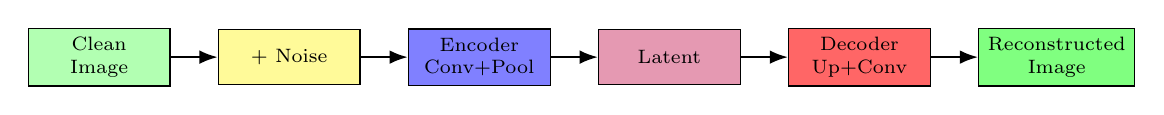
\begin{tikzpicture}[
				layer/.style={draw, minimum width=1.8cm, minimum height=0.7cm, align=center, font=\scriptsize},
				arrow/.style={-Latex, thick}
			]
			% Input
			\node[layer, fill=green!30] (clean) {Clean\\Image};
			\node[layer, fill=yellow!40, right=0.6cm of clean] (noise) {+ Noise};
			\node[layer, fill=blue!50, right=0.6cm of noise] (enc) {Encoder\\Conv+Pool};
			\node[layer, fill=purple!40, right=0.6cm of enc] (latent) {Latent};
			\node[layer, fill=red!60, right=0.6cm of latent] (dec) {Decoder\\Up+Conv};
			\node[layer, fill=green!50, right=0.6cm of dec] (recon) {Reconstructed\\Image};

			% Arrows
			\draw[arrow] (clean) -- (noise);
			\draw[arrow] (noise) -- (enc);
			\draw[arrow] (enc) -- (latent);
			\draw[arrow] (latent) -- (dec);
			\draw[arrow] (dec) -- (recon);
		\end{tikzpicture}
	}
\end{center}

\section{Generative Models}

There are two primary objectives:

\subsection*{Probabilistic Interpretation}
\[
	\begin{aligned}
		E(x) & \approx P_{\theta_E}(z \mid x)                                         & \quad & \text{(Encoder approximates the posterior of latent variables)} \\
		D(z) & \approx P_{\theta_D}(x \mid z)                                         & \quad & \text{(Decoder models the likelihood of data given latents)}    \\
		P(x) & = \int \int P(x \mid \theta, \phi) P(\theta, \phi) \, d\theta \, d\phi & \quad & \text{(Marginal likelihood of the data)}
	\end{aligned}
\]

\subsection*{Reconstruction Objective}
\[
	\mathcal{L}_{\text{recon}} = \mathbb{E}_{z \sim E(x)} \big[ \| x - D(z) \|^2 \big]
\]

\question{
	So far we have not enforced any ``structure'' on the latent $\vec{z}$. Without structure, we cannot generate \textit{new images} from $D()$, because we do not know which latent vectors to sample.

	For example, how would you pick $\vec{z}$ to generate an image of an orange-tabby cat?}

\section{Variational Autoencoder (VAE)}

To enable generative modeling, we enforce a prior distribution on the latent space, typically Gaussian:
\[
	\vec{z} \sim \mathcal{N}(0, I)
\]

Properties of Gaussian latent spaces:
\begin{itemize}
	\item Isotropic: covariance matrix is $I$
	\item Dimensions are independent
	\item Any linear combination of $\vec{z}$ preserves the Gaussian structure
\end{itemize}

VAEs provide a probabilistic interpretation of autoencoders, allowing us to sample from the model to generate new data. Assume training data $\{ x^i \}_{i=1}^N$ and latent variables $z$.

\subsection*{Data Likelihood}
\[
	p_\theta(x) = \int p_\theta(z) \, p_\theta(x|z) \, dz \approx \frac{p_\theta(x|z)p_\theta(z)}{p_\theta(z|x)}
\]

\subsection*{Evidence Lower Bound (ELBO)}
\[
	\log p(x^i) = \mathbb{E}_{z \sim q_\phi(z|x^i)} \Big[ \log p_\theta(x^i|z) \Big] - D_{\text{KL}} \big( q_\phi(z|x^i) \, \| \, p_\theta(z) \big)
\]

Where:
\begin{itemize}
	\item $q_\phi(z|x)$: encoder approximating the posterior
	\item $p_\theta(x|z)$: decoder likelihood
	\item $D_{\text{KL}}$: KL divergence regularizes the latent space to match the prior
\end{itemize}

\subsection*{VAE Computation Flow}
\[
	\begin{gathered}
		x \rightarrow (\mu_{z|x}, \Sigma_{z|x}) \rightarrow z \sim \mathcal{N}(\mu_{z|x}, \Sigma_{z|x}) \\
		z \rightarrow (\mu_{x|z}, \Sigma_{x|z}) \rightarrow \hat{x}
	\end{gathered}
\]

\end{document}
